\documentclass[11pt]{article}
\usepackage[sc]{mathpazo} %Like Palatino with extensive math support
\usepackage{fullpage}
\usepackage[authoryear,sectionbib,sort]{natbib}
\linespread{1.7}
\usepackage[utf8]{inputenc}
\usepackage{lineno}
\usepackage{titlesec}
\titleformat{\section}[block]{\Large\bfseries\filcenter}{\thesection}{1em}{}
\titleformat{\subsection}[block]{\Large\itshape\filcenter}{\thesubsection}{1em}{}
\titleformat{\subsubsection}[block]{\large\itshape}{\thesubsubsection}{1em}{}
\titleformat{\paragraph}[runin]{\itshape}{\theparagraph}{1em}{}[. ]\renewcommand{\refname}{Literature Cited}
% my addnl packages
\usepackage{geometry}
\usepackage{graphicx}
\usepackage[T1]{fontenc}
\usepackage[utf8]{inputenc}
\usepackage{authblk}
\usepackage{setspace}
\usepackage{amsfonts,amssymb,amsmath,hyperref}
\usepackage{float}
\usepackage{caption}
\usepackage{multirow}
\usepackage{hyperref}
\usepackage{wrapfig}
\usepackage{rotating}
\usepackage[usenames,dvipsnames]{xcolor}
\newcommand{\revise}[1]{{\color{Mahogany}{#1}}}
\usepackage[normalem]{ulem}
\newcommand{\tom}[2]{{\color{red}{#1}}\footnote{\textit{\color{red}{#2}}}}

\doublespacing
%\bibliography{creosote_SIPM}


%-------------------------------------------------------------------------

\title{Variation in the demographic effects of grass-endophyte symbiosis and endophyte hyphal density across an aridity gradient}

\author[1]{Jacob K. Moutouama$^{\ast}$}
\author[1]{Julia Martin}
\author[1]{Ulisses Rizo}
\author[1]{Malcolm Sherwood}
\author[1]{Emily Chong}
\author[1]{Dajanae Pearson}
\author[1]{Alexandra Jimenez Martín}
\author[2]{Josh Fowler}
\author[1]{Ali Campbell}
\author[1]{Chris Oxley}
\author[1]{Karl Schrader}
\author[1]{Tom E.X. Miller}
\affil[1]{Program in Ecology and Evolutionary Biology, Department of BioSciences, Rice University, Houston, TX USA}
\affil[2]{University of Miami, Department of Biology, Miami, Florida}

%-------------------------------------------------------------------------
\usepackage{Sweave}
\begin{document}
\maketitle
\noindent{} $\ast$ Corresponding author: jmoutouama@gmail.com\\
\noindent{} Manuscript type: Article\\
\noindent{} Open Research statement: All data X used in this paper are  publicly avaialbale. Should the paper be accepted, all computer scripts supporting the results will be archived in a Zenodo package, with the DOI included at the end of the article. During peer review, our data and code are available at \url{https://github.com/jmoutouama/ELVI-endophyte-density}. 

%\SweaveOpts{concordance=TRUE}

\linenumbers

%-------------------------------------------------------------------------
\newpage
\section*{Abstract}

%-------------------------------------------------------------------------
\section*{Keywords}

density-dependence, ecotones, woody encroachment, shrubs, integral projection model, dispersal, Allee effects

%--------------------------------------------------------------------
\newpage
\section*{Introduction}
Plant-microbe symbioses are widespread and ecologically important. 
These interactions are famously context-dependent, where the direction and strength of the interaction outcome depends on the environment in which it occurs \textcolor{violet} {(Fowler et al. 2023)}.
On the one hand endophyte symbiosis can benefits host plants by enhancing host resistance to abiotic stress such as drought, competitive ability, and resistance to herbivory and diseases.
One the other hand, endophyte symbiosis can also be detrimental to host species by reducing host biomass or reproduction under nutrient poor conditions. 
These context-dependent costs and benefits may ultimately underlie the observed distribution of host species. 

P2: Context-dependence raises the hypothesis that plant-microbe interactions are likely to vary across environmental gradients spanning range-core to range-edge. 
If the benefits of microbial symbiosis strengthen under environmental stress then symbionts could make range-edge environments more suitable, possibly extending the host’s range limits. 

P3. Ecological studies of plant-microbe symbiosis usually study the interaction from the plant’s perspective. 
Much less is known about how dynamics of the symbiont respond to environmental variation, and how this might translate to its influence on host performance. 

P4: We studied the symbiotic association between a cool-season grass species (Elymus virginicus) and its vertically transmitted fungal symbiont Epichloë elymi. [Describe ecology and natural history of grass-endophyte interactions]

P5: Working across a precipitation gradient in the south-central US, we asked how the demographic effects of endophyte symbiosis varied from core to edge of the host range.
We also quantified fungal growth in planta from range core to range edge. 
Our experiment was design to test the following hypotheses:

We hypothesized that stress associated with aridity and low precipitation would strengthen the plant-fungal mutualism, such that the fitness benefits of endophyte symbiosis are maximized at the range edge. 

We hypothesized that fungal growth in planta varied from range core to range edge. If endophyte growth is limited by host photosynthesis, then environments that are stressful for hosts may correspond to poor endophyte growth. Alternatively, if active regulation by the host is required to keep symbionts “in check”, then environments that are stressful for hosts may correspond to high endophyte growth.


%--------------------------------------------------------------------
\section*{Materials and methods}

\subsection*{Study species}
\emph {Elymus virginicus} (Virginia wildrye) is a C3 perennial bunchgrass native to woodland and prairie habitats of eastern North America. 
The westernmost range limits of this species correspond to the longitudinal aridity gradient in the central and southern Great Plains (Figure 1). 
The life cycle of \emph{E. virginicus}is typical of cool-season grasses, with seed germination in winter, growth in spring, and seed production in early summer. 
We measure plant size as a count of vegetative tillers. Reproducing plants produce spikelet-bearing inflorescences, and each spikelet typically produces 2-3 seeds. 
This species is capable of both self-pollination and outcrossing \textcolor{violet}{(Sneck et al. 2019)}. 
Throughout its range, \emph {E. virginicus} is commonly symbiotic with the seed-transmitted fungal endophyte Epichloë elymi (Clavipitaceae). 
In a prior study across natural populations in Texas, endophyte prevalence (fraction of plants that are endophyte-symbiotic) ranged from 10\% to 100 \%, with a mean of 53 \% \textcolor{violet}{(Sneck et al. 2017)}. 
Fungal genotyping indicated that the endophytes are capable of synthesizing peramine, loline, and ergot alkaloids, which may confer resistance against drought and herbivory \textcolor{violet}{(Sneck et al. 2017)}.

\subsection*{Common garden experiment}
\paragraph {Source material, identification of indiviudal endophyte status and experimental Design} 
We established a common garden experiment at 7 sites across the geographic range of \emph {Elymus virginicus} (fig.\ref{fig:site}). 
Experimental sites spanned a aridity gradient (temperature gradient in addition to the soil moisture gradient)
From the time the plants were placed on the ground to the time we collected demographic data, hourly temperature and soil moisture at each site using the HOBO MX2307 data loggers. 
We used this hourly variable to calculate the daily mean temperature ($\deg$C) and soil moisture (\%)(fig.\ref{fig:gradient}). 
% We calculated the mean soil moisture and the coefficient of variation from the time the plants were placed on the ground to the time we collected demographic data. 
The coefficient of variation of soil moisture was estimated to capture season variability in climatic data. 
The common garden experiment used E. virginicus plants that were derived from natural populations throughout the native range in the south-central US (fig.\ref{fig:site}, Table X). 
At each of these natural populations we collected seeds. 
These seeds were planted at Rice University greenhouse on Happy Frog Potting Soil (Samoa, CA) in 3.8 cm ✕ 14 cm (107 ml volume) containers.
Seedlings were regularly fertilized (Miracle-Gro Liquid All Purpose Plant Food Concentrate) every two weeks. 
To reach the target numbers for each population, we opted to employ vegetative cloning of the greenhouse-grown plants in order to achieve our desired quantity (N = 840).

Before planting in the field, we confirmed the endophyte status of all individuals using either microscopy or an immunoblot assay. This was necessary due to the varying success of the heat treatment and differences in the prevalence of endophytes between the natural populations. Leaf tissues were stained with aniline blue lactic acid and viewed under a compound microscope at 200x-400x to identify fungal hyphae. The immunoblot assay (Phytoscreen field tiller endophyte detection kit, Agrinostics Ltd. Co.) uses monoclonal antibodies that target proteins of Epichloë spp. and chromagen to visually indicate presence or absence. Both methods yield similar detection rates.  

Common gardens were established in 8 plots per site. 
Plots were 1.5m X 1.5m and the area was tilled of existing vegetation to control for native plant competition.
Plots were also selected in shaded areas under tree canopy or near shrubs to mimic the natural environmental of the species.
For each plot, we randomly assigned a starting endophyte frequency (80\%, 60\%, 40\%, 20\%, N = 2 for each endophyte frequency, N = 15 plants per plot) and herbivory treatment (herbivory excluded and control, N = 4 for each herbivory treatment). 
In each plot, we planted the \emph{E. virginicus} approximately 15 cm deep in an evenly spaced 4✕4 grid pattern, with positions randomly assigned. 
We ensured that all plots had comparable quantities of populations and genotypes between endophyte statuses and  \textcolor{red} {herbivory treatments and that plants had reached similar growth stages}.
The vegetatively cloned plants were distributed across all sites intentionally to allow for comparison of endophyte hyphae densities. 
After establishing the plot, we watered the plants and recorded initial tiller counts, flowering status and plot position so that the endophyte status, source population, and genotype of each individual plant was documented. 
\textcolor{red} {For herbivory exclusion plots, we enclosed them with 1.2m tall mesh fencing to prevent browsing by vertebrate herbivores and sprayed the plots with insecticide (Sevin Insect Killer Concentrate). 
For herbivory control plots, we half enclosed the plots with the mesh netting to control for the presence of fencing.}
We stationed one HOBO MX2307 data logger at each site to collect temperature and volumetric water content in the soil every hour. 



\subsection*{Demographic data}
We collected demographic data including survival, growth, and reproduction during June 2023, which coincided with the flowering season of \emph{E. virginicus}. 
On each individual, survival of plants was recorded as a binary (death or alive) and the size of the plant was recorded as the number of living tillers, indicated by the presence of green coloration. 
We recorded the number of inflorescences per plant and the number of spikelets on up to three inflorescences from three reproducing plants.
We limited the spikelets count to three reproducing tillers per plot due to the time consuming nature of this measurement process. 
We used the number of spikelets for these three tillers to estimate the number the average number of spikelets per plants.


\subsubsection*{Endophyte density measurements}
We collected leaf samples from E+ genotypes that were clonally replicated across two or more sites to quantify endophyte hyphal density and test its associations with host genotype and environmental factors. 
Relying on clonally replicated genotypes for this analysis allowed us to observe the same genetic individuals in different environments, and partition variation in symbiont density between genetic and environmental sources. 

There were seven unique genotypes of E+ hosts (three PALM, three JLP, one SHS) that were clonally replicated across two or more experimental sites. 
We collected leaf samples from clonal replicates of these genotypes at up to five sites (excluding COL and SON, where no samples were taken) at the time of the demographic census.
Samples were taken opportunistically based on survival status and size (we avoided leaf collection from small individuals with few leaves that were vulnerable to mortality).
We collected 20 leaf samples in total, consisting of one genotype replicated at five sites, three genotypes replicated at three sites, and three genotypes replicated at two sites. 

Samples were placed in a cold cooler in the field and then stored in a -20 freezer until processing.
In the lab, we examined sections of inner leaf sheath for hyphal density. 
For each sample, four “peels” of the leaf sheath were placed on a single gridded glass slide (including xmm cells), stained with an aniline blue-lactic acid solution, and viewed under a light microscope at X magnification, following methods in \textcolor{violet}{Sneck et al. 2019}. 
We randomly sub-sampled cells on the gridded slide, skipping those with less than 25\% leaf peel coverage, until we reached 10 cells for each sample, which amounted to a subsample totaling up to 12mm² per leaf.
We took digital images of each grid cell. 
Using ImageJ, we set the scale using the microscope reticle to measure the visible area of the leaf peel within the cell and the total length of the hyphae fragments within the leaf peel.
This yielded an estimate of endophyte density in the units of length (mm) per area (mm2). 

\subsubsection*{Host demography analysis}
To assess how stress associated with aridity and low precipitation affect plant-fungal mutualism, we developed five mixed-effects models for each vital rate. 
Each vital rate was modeled with 10 candidates models. 
These included XXX

In each of the mixed-effects models, we specified two random effects to account for heterogeneity among plot within site and heterogeneity among host source populations. The first random effect was a nested random effect (plot within site) and the second one was a random intercept effect (population). We modeled growth with a Gaussian distribution using the package lmertest  \textcolor{blue}{(Source)}. We modeled fertility (number of spikelet) with a zero-inflated negative binomial distribution using the package glmmTMB  \textcolor{blue}{(Source)}. We preferred the negative binomial in which the variance was modeled as a non-linear function of the mean (variance = m (1 + m/k)). For each vital rate, the first model was the intercept only model which is the null model. The second and the third models regressed vital rate against the additive effect of endophyte status and mean of soil moisture or coefficient of variation of soil moisture. The fourth and fifth models regressed vital rates against the interaction effect of endophyte status and mean of soil moisture or coefficient of variation of soil moisture (Appendix S1). We compared the five models using the Akaike Information Criterion (AIC) to select the best model \textcolor{blue}{(Source)}. 

\subsubsection* {Symbiont density analysis}
For the subset of E+ plants sampled for endophyte hyphal density, we used AIC-based model selection to quantify support for genetic and environmental influences on symbiont density. We fit mixed models with a Gaussian error distribution using the natural log of endophyte density as the response variable. All sampled plants had been previously assessed as E+ but a few leaf peel samples had no detectable endophytes. We therefore added an arbitrarily small constant value to the density measurements (0.1) to avoid log(0). All models used the 10 subsamples as raw data and included the individual ID as a random effect. 

We analyzed endophyte density with two complementary approaches. In the first set of four candidate models we included host-symbiont genotype, experimental site, neither, or both as explanatory fixed-effect variables (Table ##). Because we did not have consistent representation of all genotypes at all sites we were not able to fit a genotype:site interaction, as would arise if different genotypes performed better at different sites. We assessed support for the candidate models using AIC, and for the model that included both genotype and site we partitioned the variance explained by each factor by deriving the marginal R2 using package partR2 \textcolor{blue}{(cite)}. Models including site capture all possible differences across sites. To explore the specific influence of soil moisture, we fit a second set of eight candidate models that included genotype and/or mean soil moisture, and genotype and/or the CV of soil moisture, including interactions. 

All  analyzes were conducted in R 4.1.3 \textcolor{blue}{(Source)}. 


%--------------------------------------------------------------------
\section*{Results}
All the best-supported stress vital rate models  included endophyte status, suggesting a strong 
effect of fungal mutualism on plant demography. Soil aridity (change in water content per day) had a large influence on individual growth rate, number of inflorescences, and number of spikelets (Fig X, Table X). However, that influence was different for endophyte-free individuals and endophyte colonized. Endophyte colonized individuals had a size advantage in a more arid condition than endophyte-free individuals in higher seasonal variation (Fig. A). In contrast, endophyte free individuals produced more spikelet under more arid conditions than endophyte colonized individuals (Fig. C). There was no difference between endophyte-free individuals and endophyte-colonized individuals in flower number (Fig. C). 

%--------------------------------------------------------------------
\section*{Discussion}





%--------------------------------------------------------------------
\section*{Acknowledgements}

\section*{Author contributions}
All authors contributed to study design. 
THD and TEXM led data analysis, modeling, and writing early drafts of the manuscript. 
All authors participated in preparing the manuscript for submission.

%--------------------------------------------------------------------
\bibliographystyle{ecology}
\bibliography{ELVI}

\newpage
\section*{Figure legends}
\begin{figure}[H]
  \begin{center}
   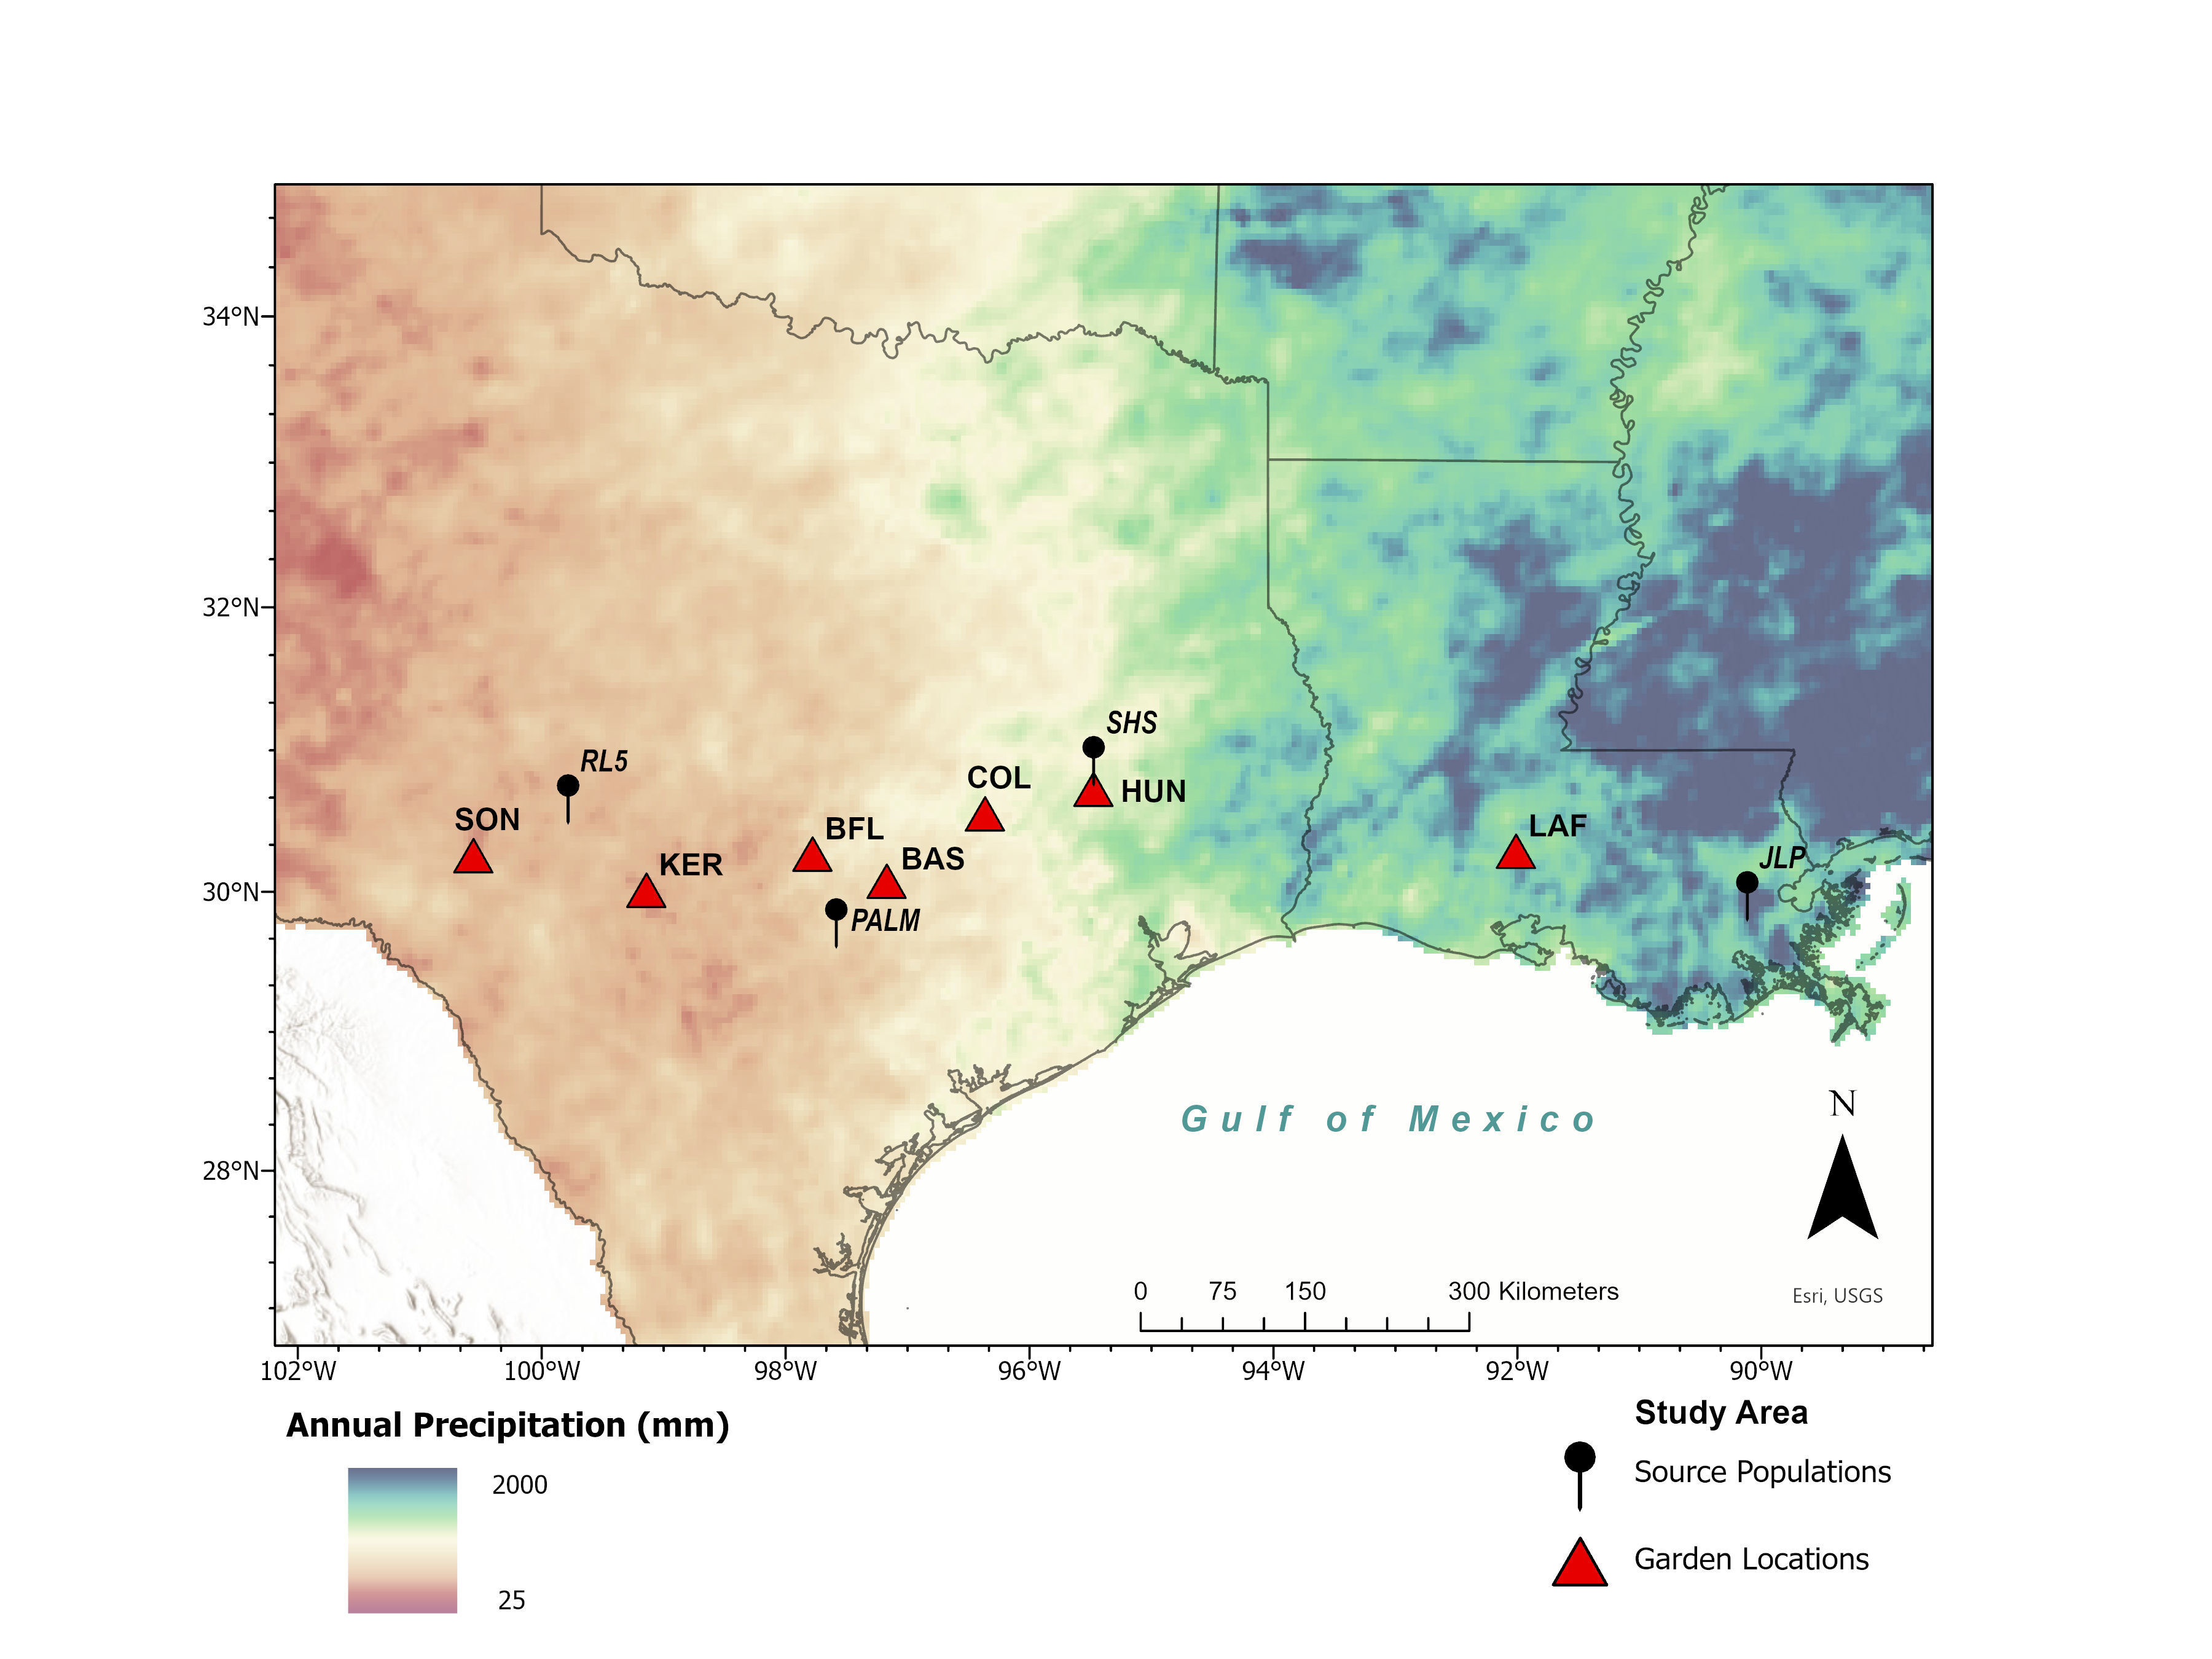
\includegraphics[width=0.99\linewidth]{Figures/Study_site.jpg}
  \caption{}
  \label{fig:site}
  \end{center}
\end{figure}

\begin{figure}[H]
  \begin{center}
   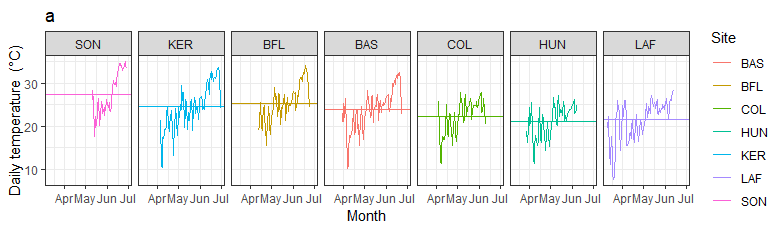
\includegraphics[width=0.98\linewidth]{Figures/Temperature.png}
  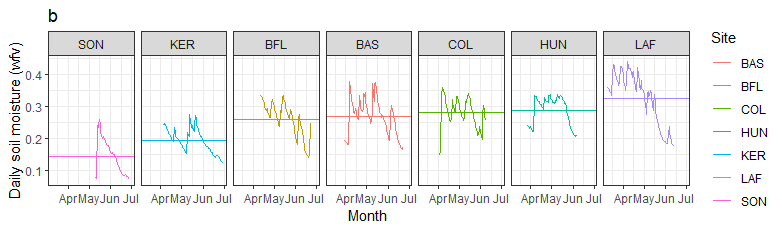
\includegraphics[width=0.98\linewidth]{Figures/Soil_moisture.png}
  \caption{}
  \label{fig:gradient}
  \end{center}
\end{figure}


\begin{figure}[H]
  \begin{center}
   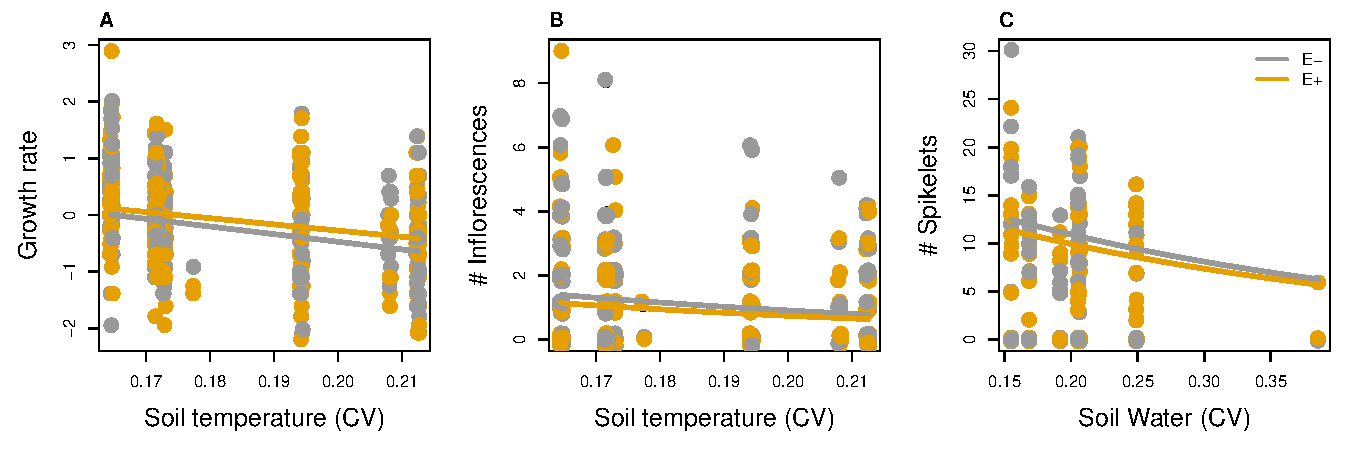
\includegraphics[width=0.98\linewidth]{Figures/Bestmodels.pdf}
  \caption{}
  \label{fig:gradient}
  \end{center}
\end{figure}


\end{document}
